\section{Statischer Verstärkungsfaktor}

Der statischer Verstärkungsfaktor des behandelten $IT_1-Gliedes$ ist $\infty$, da ein integrierendes Verhalten vorliegt. Der Graph der Übergangsfunktion strebt gegen unendlich. \\ \\
Nichtsdestotrotz lässt sich feststellen, dass die Übergangsfunktion die Asymptote \[y = 4x\] besitzt bzw. dass die Gewichtsfunktion gegen den Wert 4 konvergiert. \\
Der Graph dieser Gerade ist in Abbildung \ref{fig:static-curve} zu sehen. Dabei sind auf der $x-Achse$ die konstanten Eingänge und auf der $y-Achse$ die Ausgänge des Systems für $t \rightarrow \infty$ aufgetragen.

\begin{figure}[H]
	\centering
	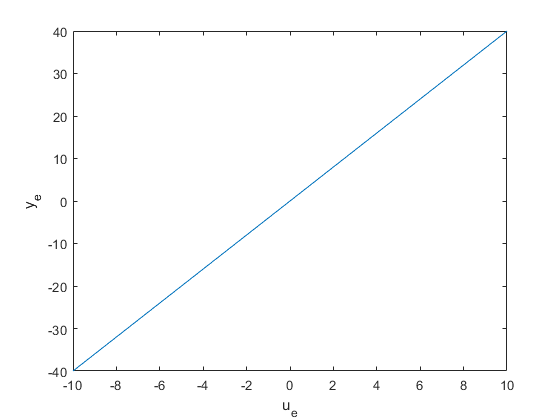
\includegraphics[width=0.7\linewidth]{{diagrams/staticCurve.png}}
	\caption[Asymptote]{Asymptote der Übergangsfunktion}
	\label{fig:static-curve}
\end{figure}